\chapter{Maxwell's equations and Conservation laws}
section{Electrodynamics Before Maxwell}
Till now in electromagnetic theory we found out four equations which contribute to the foundation of Electromagnetic theory, and they are,
\begin{align*}{2}
\vec{\nabla} \cdot \vec{E}&=\frac{\rho}{\epsilon_{0}} \quad && \Rightarrow \text { Gauss' Law }  \\
\vec{\nabla} \cdot \vec{B}&=0 \quad && \Rightarrow \text { Gauss' Law for magnetism } \\
\vec{\nabla} \times \vec{E}&=-\frac{\partial \vec{B}}{\partial t} && \Rightarrow \text { Faraday's Law } \\
\vec{\nabla} \times \vec{B}&=\mu_{0}\left(\vec{J}\right) && \Rightarrow \text { Ampere's Law }
\end{align*}
There is a fatal inconsistency in these formulas. It has something to do with the old rule that divergence of curl is always zero $ (\nabla .(\nabla \times E)=0)$. If you apply the divergence to Faraday's law, everything works out: 
$$\nabla \cdot(\nabla \times \mathbf{E})=\nabla \cdot\left(-\frac{\partial \mathbf{B}}{\partial t}\right)=-\frac{\partial}{\partial t}(\nabla \cdot \mathbf{B})$$
The left side is zero because divergence of curl is zero; the right side is zero by virtue of Gauss law for magnetism. But when you do the same thing to Ampere's law, you get into trouble:$$\boldsymbol{\nabla} \cdot(\boldsymbol{\nabla} \times \mathbf{B})=\mu_{0}(\boldsymbol{\nabla} \cdot \mathbf{J})$$ The left side must be zero, but the right side, in general, is not. For steady currents, the divergence of $\mathbf{J}$ is zero, but evidently when we go beyond magnetostatics Ampère's law cannot be right.
\subsection{How Maxwell Fixed Ampère's Law}
Applying the continuity equation  and Gauss's law, in  Ampere's law the offending term can be rewritten as:
\begin{align*}
\nabla \cdot \mathbf{J}&=-\frac{\partial \rho}{\partial t}\\
&=-\frac{\partial}{\partial t}\left(\epsilon_{0} \nabla \cdot \mathbf{E}\right)\\&=-\nabla \cdot\left(\epsilon_{0} \frac{\partial \mathbf{E}}{\partial t}\right)
\end{align*}
If we were to combine $\epsilon_{0}(\partial \mathbf{E} / \partial t)$ with $\mathbf{J}$, in Ampère's law, it would be just right to kill off the extra divergence:$$\nabla \times \mathbf{B}=\mu_{0} \mathbf{J}+\mu_{0} \epsilon_{0} \frac{\partial \mathbf{E}}{\partial t}$$ Such a modification changes nothing, as far as magnetostatics is concerned: when $\mathbf{E}$ isconstant, we still have $\boldsymbol{\nabla} \times \mathbf{B}=\mu_{0} \mathbf{J}$.\\
Just as a changing magnetic field induces an electric field (Faraday's law), so \textbf{A changing electric field induces a magnetic field}.  Maxwell called his extra term the displacement current:

\hspace{5.10cm}\framebox{
	
	\parbox[t][1.5cm]{4cm}{
		
		\addvspace{0.2cm} \centering 
		Displacement Current\\\vspace{0.2cm}
		$\mathbf{J}_{d} \equiv \epsilon_{0} \frac{\partial \mathbf{E}}{\partial t}$} 
}
\\\\ It's a misleading name, since $\epsilon_{0}(\partial \mathbf{E} / \partial t)$ has nothing to do with current, except that it adds to $\mathbf{J}$ in Ampère's law.
\subsection{Maxwell's Equations}
\begin{center}
	\framebox{
		\parbox[t][4.2cm]{3.5cm}{
			
			\addvspace{0.2cm} \centering
			
			\begin{align*}
			\begin{array}{lll}
			\textbf{(i)} & \nabla \cdot \mathbf{E}=\frac{1}{\epsilon_{0}} \rho&\text{(Gauss's law)} \\\\ \textbf{(ii)} & \nabla \cdot \mathbf{B}=0&\text{(No name.)}\\\\ \textbf{(iii)}& \boldsymbol{\nabla} \times \mathbf{E}=-\frac{\partial \mathbf{B}}{\partial t}&\text{(Faraday's law)}\\\\\textbf{(iv)}&\boldsymbol{\nabla} \times \mathbf{B}=\mu_{0} \mathbf{J}+\mu_{0} \epsilon_{0} \frac{\partial \mathbf{E}}{\partial t}&\text{(Ampère's law with
				Maxwell's correction)}
			\end{array}
			\end{align*}} }
\end{center}
Every phenomenon in electricity and magnetism can be derived from these equations. Many of our most important tools for various analyses come from the integral version of these equations, which are.
\begin{center}
	\framebox{
		\parbox[t][4.2cm]{3.5cm}{
			
			\addvspace{0.2cm} \centering
			
			\begin{align*}
			\begin{array}{lll}
			\textbf{(i)} & \iint_{S} \overrightarrow{\mathbf{E}} \cdot d \overrightarrow{\mathbf{A}}=\frac{Q}{\varepsilon_{0}} &\text{(Gauss's law)} \\\\ \textbf{(ii)} & \iint_{S} \overrightarrow{\mathbf{B}} \cdot d \overrightarrow{\mathbf{A}}=0&\text{(No name.)}\\\\ \textbf{(iii)}& \oint \overrightarrow{\mathbf{E}} \cdot d \overrightarrow{\mathbf{s}}=-\frac{d \mathbf{\phi_B}}{d t}&\text{(Faraday's law)}\\\\\textbf{(iv)}&\oint \overrightarrow{\mathbf{B}} \cdot d \overrightarrow{\mathbf{s}}=\mu_{0} I+\mu_{0} \varepsilon_{0} \frac{d \Phi_{E}}{d t}&\text{(Ampère's law with
				Maxwell's correction)}
			\end{array}
			\end{align*}} }
\end{center} 
Together with the force law,\ $\mathbf{F}=q(\mathbf{E}+\mathbf{v} \times \mathbf{B})$,\ they summarize the entire theoretical content of classical electrodynamics. Even the continuity equation,\ $\boldsymbol{\nabla} \cdot \mathbf{J}=-\frac{\partial \rho}{\partial t}$ \ which is the mathematical expression of conservation of charge, can be derived from Maxwell's equations by applying the divergence to Ampere's law.
\subsection{Maxwell's Equations In Free Space}
An extremely important limit of Maxwell's equations is found when there are no sources: $\rho=0, \vec{J}=0 .$ The equations become,
\begin{center}
	\framebox{
		\parbox[t][4.2cm]{3.5cm}{
			
			\addvspace{0.2cm} \centering
			
			\begin{align*}
			\begin{array}{lll}
			\textbf{(i)} & \nabla \cdot \mathbf{E}=0&\text{(Gauss's law)} \\\\ \textbf{(ii)} & \nabla \cdot \mathbf{B}=0&\text{(No name.)}\\\\ \textbf{(iii)}& \boldsymbol{\nabla} \times \mathbf{E}=-\frac{\partial \mathbf{B}}{\partial t}&\text{(Faraday's law)}\\\\\textbf{(iv)}&\boldsymbol{\nabla} \times \mathbf{B}=\mu_{0} \epsilon_{0} \frac{\partial \mathbf{E}}{\partial t}&\text{(Ampère's law with
				Maxwell's correction)}
			\end{array}
			\end{align*}} }
\end{center}
\subsection{Maxwell's Equations in Matter}
For inside polarized matter there will be accumulations of "bound" charge and current over which you exert no direct control. It would be nice to reformulate Maxwell's equations in such a way as to make explicit reference only to those sources we control directly: the "free" charges and currents. \\
We have already learned, from the static case, that an electric polarization $\mathbf{P}$ produces a bound charge density $$\rho_{b}=-\nabla \cdot \mathbf{P}$$ Likewise, a magnetic polarization (or "magnetization") $\mathbf{M}$ results in a bound current $$\mathbf{J}_{b}=\nabla \times \mathbf{\mathbf { M }}$$ There's just one new feature to consider in the nonstatic case: Any change in the electric polarization involves a flow of (bound) charge (call it $\mathbf{J}_{p}$), which must be included in the total current. For suppose we examine a tiny chunk of polarized material The polarization introduces a charge density $\sigma_{b}=P$ at one end and $-\sigma_{b}$ at the other. If $P$ now increases a bit, the charge on each end increases accordingly. \\giving a net current $$d I=\frac{\partial \sigma_{b}}{\partial t} d a_{\perp}=\frac{\partial P}{\partial t} d a_{\perp}$$
\begin{figure}[H]
	\begin{center}
		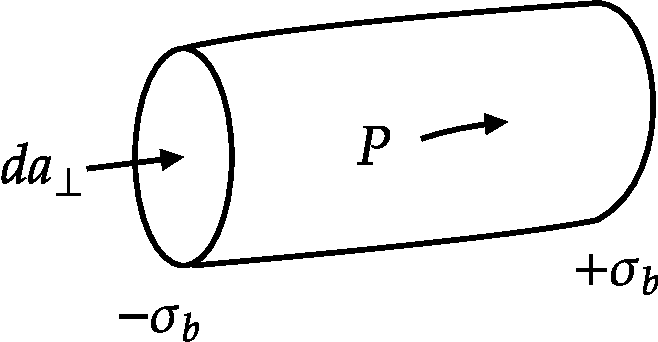
\includegraphics[width=4cm,height=2cm]{02-crop}
	\end{center}
\end{figure}
The current density, therefore, is $$\mathbf{J}_{p}=\frac{\partial \mathbf{P}}{\partial t}$$
This polarization current has nothing whatever to do with the bound current $\mathbf{J}_{b}$. The latter is associated with magnetization of the material and involves the spin and orbital motion of electrons; $\mathbf{J}_{p}$, by contrast, is the result of the linear motion of charge when the electric polarization changes. If $\mathbf{P}$ points to the right and is increasing, then each plus charge moves a bit to the right and each minus charge to the left; the cumulative effect is the polarization current $\mathbf{J}_{p}$\\\\
In fact, $\mathbf{J}_{p}$ is essential to account for the conservation of bound charge.\\
In view of all this, the total charge density can be separated into two parts: $$\rho=\rho_{f}+\rho_{b}=\rho_{f}-\boldsymbol{\nabla} \cdot \mathbf{P}$$ and the current density into three parts:
$$\mathbf{J}=\mathbf{J}_{f}+\mathbf{J}_{b}+\mathbf{J}_{p}=\mathbf{J}_{f}+\mathbf{\nabla} \times \mathbf{M}+\frac{\partial \mathbf{P}}{\partial t}$$ Gauss's law can now be written as $$\nabla \cdot \mathbf{E}=\frac{1}{\epsilon_{0}}\left(\rho_{f}-\nabla \cdot \mathbf{P}\right)$$ \text{or}$$\boldsymbol{\nabla} \cdot \mathbf{D}=\rho_{f}$$ where $\mathbf{D}$, as in the static case, is given by $$\mathbf{D} \equiv \epsilon_{0} \mathbf{E}+\mathbf{P}$$ Meanwhile, Ampère's law (with Maxwell's term) becomes $$\nabla \times \mathbf{B}=\mu_{0}\left(\mathbf{J}_{f}+\nabla \times \mathbf{M}+\frac{\partial \mathbf{P}}{\partial t}\right)+\mu_{0} \epsilon_{0} \frac{\partial \mathbf{E}}{\partial t}$$\text{or}$$\boldsymbol{\nabla} \times \mathbf{H}=\mathbf{J}_{f}+\frac{\partial \mathbf{D}}{\partial t}$$ where, as before,$$\mathbf{H} \equiv \frac{1}{\mu_{0}} \mathbf{B}-\mathbf{M}$$ Faraday's law and $\nabla \cdot \mathbf{B}=0$ are not affected by our separation of charge and current into free and bound parts, since they do not involve $\rho$ or $\mathbf{J}$. \\
In terms of free charges and currents, then, Maxwell's equations read\
\begin{center}
	\framebox{
		\parbox[t][2.5cm]{4cm}{
			
			\addvspace{0cm} \centering
			
			\begin{align*}
			\begin{array}{llll}
			\textbf{(i)} & \nabla \cdot \mathbf{D}=\rho_{f} &\textbf{(iii)} & \boldsymbol{\nabla} \times \mathbf{E}=-\frac{\partial \mathbf{B}}{\partial t},\\\\
			\textbf{(ii)}&\boldsymbol{\nabla} \cdot \mathbf{B}=0&\textbf{(iv)}& \boldsymbol{\nabla} \times \mathbf{H}=\mathbf{J}_{f}+\frac{\partial \mathbf{D}}{\partial t}
			\end{array}
			\end{align*}} }
\end{center}
for linear media
\begin{align*}
\begin{array}{lll}
\mathbf{P}=\epsilon_{0} \chi_{e} \mathbf{E} & and& \mathbf{M}=\chi_{m} \mathbf{H}\\\\
\mathbf{D}=\epsilon \mathbf{E}&and&\mathbf{H}=\frac{1}{\mu} \mathbf{B}
\end{array}
\end{align*}
where $\epsilon \equiv \epsilon_{0}\left(1+\chi_{e}\right)$ and $\mu \equiv \mu_{0}\left(1+\chi_{m}\right)$ D is called the electric "displacement"; that's why the second term in the Ampère/Maxwelf equation (iv) is called the displacement current,\\
In integral form Maxwell's equations in matter can be written as\\
\begin{align*}
\text{(i)}\hspace{0.5cm}\oint_{s}D\cdot da&=\theta_{fenc}\\
\text{(ii)}\hspace{0.5cm}\oint_{s}B\cdot da&=0\\
\text{(iii)}\hspace{0.5cm}\oint_{p}E\cdot dl&=\frac{-d}{dt}\int_{s} B\cdot da\\
\text{(iv)}\hspace{0.5cm}\oint_{p}H\cdot dl&=I_{end}+\frac{d}{dt}\int_{s} D\cdot da\\
\end{align*}
$P$ is the closed loop enclosing the surface $S$
\section{Boundary conditions}
In general the fields \textbf{E,B,D,} and \textbf{H} will be discontineous at a boundary between two different media or at surface that carries charge density $\sigma$ or current density \textbf{K}. The explicit form of the discontinities can be deduced from Maxwell's equations,in their integral form\\\\
(i) $\oint_s \mathbf{D} \cdot d \mathbf{a}=Q_{f_{\mathrm{enc}}}$\\
(ii) $\oint_s \mathbf{B} \cdot d \mathbf{a}=0$\\
$\left.\begin{array}{l|l}\text { (iii) } \oint_l \mathbf{E} \cdot d \mathbf{l} & =-\frac{d}{d t} \int_s \mathbf{B} \cdot d \mathbf{a} \\ 
\text { (iv) } \oint_l \mathbf{H} \cdot d \mathbf{l} & =I_{f_{\text {enc }}}+\frac{d}{d t} \int_s \mathbf{D} \cdot d \mathbf{a}\end{array}\right\} \begin{aligned}&\text { for any surface } s \\&\text { bounded by the } \\&\text { closed loop } l .\end{aligned}$\\
Applying (i) to a tiny, wafer-thin Gaussian pillbox extending just slightly into the material on either side of the boundary, we obtain \\
\begin{figure}[H]
	\centering
	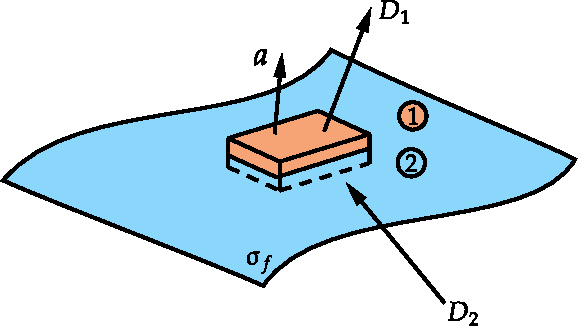
\includegraphics[height=4cm,width=7cm]{diagram-20220103(8)-crop}
	\caption{}
	\label{}
\end{figure}
$$\mathbf{D}_{1} \cdot \mathbf{a}-\mathbf{D}_{2} \cdot \mathbf{a}=\sigma_{f} a$$
Thus ,the component of D that is perperdicular to the interface is discontineous in the amount \\
$$D_{1}^{\perp}-D_{2}^{\perp}=\sigma_{f}$$
Identical reasoning,applied to equation(ii) yields\\
$$B_1^{\perp}-B_2^{\perp}=0$$
consider equation(iii) a very thin Amperian loop straddling the surface gives\\
\begin{figure}[H]
	\centering
	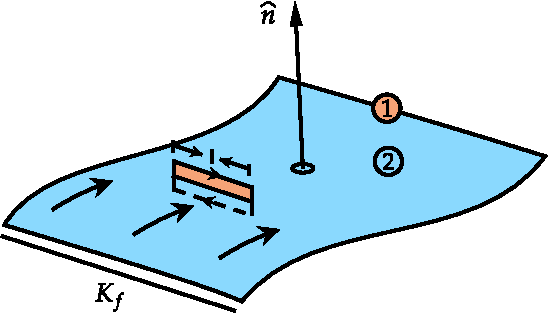
\includegraphics[height=4cm,width=7cm]{diagram-20220103(9)-crop}
	\caption{}
	\label{}
\end{figure}
$$E_1\cdot L-E_2\cdot L=-\frac{d}{dt} \int_{s} B\cdot da$$
But in the limit as the width of the loop goes to zero ,the flux vanishes.Therefore\\
$$E_1^{\parallel}-E_2^{\parallel}=0$$
That is the comonents of E parallel to the interface are contineous across the boundary.\\
equation (iv)  implies \\
$$H_1 \cdot L-H_2\cdot L=I_{f_{enc}}$$
Where $I_{f_{enc}}$ is the free current passing through the Amperian loop.No volume current density will contribute but a surface current can . In fact if $\hat{n}$ is a unit vector perpendicular to the interface so that $(\hat{n}\times L)$ is normal to the Amperian loop then,
$$I_{f_{enc}}=K_f \cdot (\hat{n}\times L)=(K_f\times \hat{n})\cdot L$$
And hence $$H_1^{\parallel}-H_2^{\parallel}=K_f\times \hat{n}$$
So the parallel components  H are discontinuous by an amount proportional to the free surface charge density.\\
In the case of linear media they can be expressed in terms of E and B alone \\\\
(i) $\epsilon_{1} E_{1}^{\perp}-\epsilon_{2} E_{2}^{\perp}=\sigma_{f}$,\\
(iii) $\mathbf{E}_{1}^{\|}-\mathbf{E}_{2}^{\|}=0$,\\
(ii) $B_{1}^{\perp}-B_{2}^{\perp}=0$,\\
(iv) $\frac{1}{\mu_{1}} \mathbf{B}_{1}^{\|}-\frac{1}{\mu_{2}} \mathbf{B}_{2}^{\|}=\mathbf{K}_{f} \times \hat{\mathbf{n}}$.\\\\
In particular, if there is no free charge or free current at the interface, then \\\\
(i) $\epsilon_{1} E_{1}^{\perp}-\epsilon_{2} E_{2}^{\perp}=0$,\\
(iii) $\mathbf{E}_{1}^{\|}-\mathbf{E}_{2}^{\|}=0$\\
(ii) $B_{1}^{\perp}-B_{2}^{\perp}=0$,\\
(iv) $\frac{1}{\mu_{1}} \mathbf{B}_{1}^{\|}-\frac{1}{\mu_{2}} \mathbf{B}_{2}^{\|}=0$.
\section{Scalar and vector potentaial}
Maxwell's equations are\\
(i) $\boldsymbol{\nabla} \cdot \mathbf{E}=\frac{1}{\epsilon_{0}} \rho$,\\
(iii) $\boldsymbol{\nabla} \times \mathbf{E}=-\frac{\partial \mathbf{B}}{\partial t}$,\\
(ii) $\boldsymbol{\nabla} \cdot \mathbf{B}=0$,\\
(iv) $\boldsymbol{\nabla} \times \mathbf{B}=\mu_{0} \mathbf{J}+\mu_{0} \epsilon_{0} \frac{\partial \mathbf{E}}{\partial t}$.\\
If $\rho(r,t)$ and $J(r,t)$ are bnown electric and magnetic field can be find out using Gauss's law and Bio-savart law.It is difficult to find E ans B if they are time dependant.To solve this problem first we are going to represents the fields in terms of potentials electric potential V and magnetic potential B.\\
In the static case $\nabla \times E=0$ So electric field cane written as a negative gradient of some scalar quandity called electric potential V\\
$$E=-\nabla V$$(not possible in elctrodynamics)\\
But $\nabla \cdot B=0$ always.Which gives \\
$$B=\nabla\times A$$
 Where A is the magnetic vector potential.Putting this value in 
$$\boldsymbol{\nabla} \times \mathbf{E}=-\frac{\partial \mathbf{B}}{\partial t}$$
We will get \\
$$\nabla \times E=\frac{-\partial }{\partial t}(\nabla \times A)$$
$$\nabla \times \left( E+\frac{\partial A}{\partial t}\right) =0$$
Again the curl of something become zero. so it can be written as negative gradient of potential
$$E+\frac{\partial A}{\partial t}=-\nabla V$$
$$E=-\nabla V-\frac{\partial A}{\partial t}$$
\begin{center}
	\framebox{
		\parbox[t][3cm]{3cm}{
			
			\addvspace{0.2cm} \centering
			
			\begin{align*}
			\begin{array}{lll}
			$$B=\nabla\times A$$\\
			$$E=-\nabla V-\frac{\partial A}{\partial t}$$
			\end{array}
			\end{align*}} }
\end{center}
If A and V are known we can find electric and magnetic field with these two equations.

Putting this equation $$E=-\nabla V-\frac{\partial A}{\partial t}$$  in Gauss's law
we will get,\\
$$\nabla ^2V+\frac{\partial }{\partial t}(\nabla \cdot A)=\frac{-\rho}{\epsilon_{0}}$$
Putting $B=\nabla\times A$  equation in Ampere/Maxwell's law and rearranging we will get,\\
$$\left( \nabla^2A-\mu_{0}\epsilon_{0}\frac{\partial^2 A}{\partial t^2}\right) -\nabla\left( \nabla \cdot A+\mu_{0}\epsilon_{0}\frac{\partial V}{\partial t}\right) =-\mu_{0} J$$ 

These two equations contain all information in the Maxwell's equations.\\
However we have succeeded in reducing six problems to find E and B ,down to four(V one component,A three component.),these equations are lengthy and difficult to find solution we have to abandon this potential formulation altogether.\\
\paragraph{Gauge transformation}
To avoid this problem we are transforming the potential equations by adding one extra term to A and V.This is called gauge tranformation.Consider the transformation occuring in the same fields E and B.Then\\
$$A^{\prime}=A+\alpha$$ and
$$V^{\prime}=V+\beta$$
Taking curl on each side of $A^{\prime}=A+\alpha$
we will get 
$$\nabla \times A^{\prime}=\nabla \times A+\nabla \times \alpha$$
Since B's are same we can written as($\nabla \times B=0,A^{\prime}=A$) \\
$$\nabla \times \alpha =0$$
Again curl of $\alpha$ is zero.then\\
$$\alpha=\nabla \lambda$$\\
The two potentials also gives the same E.so,\\
$$\nabla \beta +\frac{\partial \alpha }{\partial t}=0$$
$$\nabla\left( \beta+\frac{\partial \lambda}{\partial t}\right) =0$$
$$\beta= -\frac{\partial \lambda}{\partial t}$$
Now transformations become,\\

\begin{center}
	\framebox{
		\parbox[t][3cm]{3cm}{
			
			\addvspace{0.2cm} \centering
			
			\begin{align*}
			\begin{array}{lll}
			 $$A^{\prime}=A+\nabla \lambda$$\\
			 $$V^{\prime}=V-\frac{\partial \lambda}{\partial t}$$
			\end{array}
			\end{align*}} }
\end{center}
\subsection{Coulomb Gauge and Lorentz gauge}
\paragraph{Coluomb gauge}
$$\nabla \cdot A=0$$ is called Coulomb gauge.\\
\paragraph{importance}
$$\nabla \cdot A=0$$ Then the equation 
$$\nabla ^2V+\frac{\partial }{\partial t}(\nabla \cdot A)=\frac{-\rho}{\epsilon_{0}}$$ become,\\
$$\nabla^2 V=\frac{-\rho}{\epsilon_{0}}$$
This is poisson's equation.From this equation V can be findout by using the formula\\
$$V(r,t)=\frac{1}{4 \pi \epsilon_0}\int \frac{\rho(r^{\prime},t)}{r}d\tau^{\prime}$$
V is easy to get but to find E we need  A also($E=-\nabla V-\frac{\partial A}{\partial t}$) which is difficult.
\paragraph{Advantage of the coulomb gauge is that the scalar potential is simply to calculate .The disadvatage is that  A is particularly difficult to calculate. }
After applying coulomb gauge to the equation 
$$\left( \nabla^2A-\mu_{0}\epsilon_{0}\frac{\partial^2 A}{\partial t^2}\right) -\nabla\left( \nabla \cdot A+\mu_{0}\epsilon_{0}\frac{\partial V}{\partial t}\right) =-\mu_{0} J$$ 
we get\\
$$\left( \nabla^2A-\mu_{0}\epsilon_{0}\frac{\partial^2 A}{\partial t^2}\right)=-\mu_{0}J+\mu_{0} \epsilon_{0}\nabla \left( \frac{\partial V}{\partial t}\right) $$
\paragraph{Lorentz gauge}
$$\nabla \cdot A =-\mu_{0} \epsilon_{0} \frac{\partial}{\partial t}V$$

 is called the lorentz gauge.\\
 This designes to eliminate the middle term of the equation
$$\left( \nabla^2A-\mu_{0}\epsilon_{0}\frac{\partial^2 A}{\partial t^2}\right) -\nabla\left( \nabla \cdot A+\mu_{0}\epsilon_{0}\frac{\partial V}{\partial t}\right) =-\mu_{0} J$$
With lorentz gauge this equation become
$$\nabla^2A-\mu_{0}\epsilon_{0}\frac{\partial^2 A}{\partial t^2}=-\mu_{0} J$$
With lorentz gauge this equation 
$\nabla ^2V+\frac{\partial }{\partial t}(\nabla \cdot A)=\frac{-\rho}{\epsilon_{0}}$
becomes
$$\nabla^2A-\mu_{0}\epsilon_{0}\frac{\partial^2 A}{\partial t^2}=\frac{-\rho}{\epsilon_{0}}$$
The virtue of the lorentz gauge is that it treats V and A on the same differential operator
$$\nabla^2-\mu_{0} \epsilon_{0}\frac{\partial ^2}{\partial t^2}\equiv \square^2  $$
 is called d'Alembertian\\
Then both equation become\\
$$\square^2V=\frac{-\rho}{\epsilon_{0}}$$
$$\square^2A=-\mu_{0} J$$
\section{Retarded Potentials}
$$\square^{2} V=-\frac{1}{\epsilon_{0}} \rho, \quad \square^{2} \mathbf{A}=-\mu_{0} \mathbf{J}$$
In static case these equation reduces to poisson's equations
$$\nabla^{2} V=-\frac{1}{\epsilon_{0}} \rho, \quad \nabla^{2} \mathbf{A}=-\mu_{0} \mathbf{J}$$
with solutions
$$V(\mathbf{r})=\frac{1}{4 \pi \epsilon_{0}} \int \frac{\rho\left(\mathbf{r}^{\prime}\right)}{r} d \tau^{\prime}, \quad \mathbf{A}(\mathbf{r})=\frac{\mu_{0}}{4 \pi} \int \frac{\mathbf{J}\left(\mathbf{r}^{\prime}\right)}{r} d \tau^{\prime}$$
$r \rightarrow$ distance from source point $\vec{r}$ to the field point $r$.\\
Imagine a electromagnetic news travels at the speed of light. In non-static case therefore, it's not the status of source right now that matters but rather its condition at some earlier time $t_r$ (retarded time) when the message left.\\
Since the message must travel a distance $r$ the delay is $r/c$
$$t_{r}=t-r / c$$
$\therefore$ Potentials become
$$V(\mathbf{r})=\frac{1}{4 \pi \epsilon_{0}} \int \frac{\rho\left(\mathbf{r}^{\prime}\right)}{r} d \tau^{\prime}, \quad \mathbf{A}(\mathbf{r})=\frac{\mu_{0}}{4 \pi} \int \frac{\mathbf{J}\left(\mathbf{r}^{\prime}\right)}{r} d \tau^{\prime}$$
$P(r^\prime,t_r)$: charge density prevailed at point $r^\prime$ at the retarded time $t_r$. Because the integrants are evaluated at the retarded time these are called retarded potentials.\\
The more distant parts of the charge distribution have earlier retarded times than nearby ones.\\
In calculating the Laplacian of $V(r,t)$\\
The integrand depends on $\vec{r}$ in two places explicitly, in the denomenator $(r=|r-r^\prime|)$ and implicitly through $t_r-t-r/c$ in neumerator 
\begin{align*}
\nabla V&=\frac{1}{4 \pi \epsilon_{0}} \int\left[(\nabla \rho) \frac{1}{r}+\rho \nabla\left(\frac{1}{2}\right)\right] d \tau^{\prime}\\
\nabla \rho&=\dot{\rho} \nabla t_{r}=-\frac{1}{c} \dot{\rho} \nabla r\\
\nabla r&=\hat{r} \text{ and } \nabla \left( \frac{1}{r}\right) =\frac{-\hat{r}}{r^2}\\
\nabla V&=\frac{1}{4 \pi \epsilon_{0}} \int\left[-\frac{\rho}{c} \frac{\hat{r}}{r}-\rho \frac{\hat{\varepsilon}}{r^{2}}\right] d \tau^{\prime}
\intertext{Taking the divergence}
\nabla^{2} V&=\frac{1}{4 \pi \epsilon_{0}} \int\left\{-\frac{1}{c}\left[\frac{\hat{\imath}}{r} \cdot(\nabla \dot{\rho})+\dot{\rho} \nabla \cdot\left(\frac{\hat{r}}{r}\right)\right]\right.
-\left.-\left[\frac{\hat{z}}{r^{2}} \cdot(\nabla \rho)+\rho \nabla \cdot\left(\frac{\hat{\varepsilon}}{r^{2}}\right)\right]\right\} d \tau^{\prime} .\\
\nabla \dot{\rho}&=-\frac{1}{c} \ddot{\rho} \nabla r=-\frac{1}{c} \ddot{\rho} \hat{r},\quad 
\nabla \cdot\left(\frac{\hat{r}}{r}\right)=\frac{1}{r^{2}} 
\intertext{whereas}
&\nabla \cdot\left(\frac{\hat{r}}{r^{2}}\right)=4 \pi \delta^{3}(r)
\intertext{So}
\nabla^{2} V&=\frac{1}{4 \pi \epsilon_{0}} \int\left[\frac{1}{c^{2}} \frac{\ddot{\rho}}{r}-4 \pi \rho \delta^{3}(r)\right] d \tau^{\prime}=\frac{1}{c^{2}} \frac{\partial^{2} V}{\partial t^{2}}-\frac{1}{\epsilon_{0}} \rho(\mathbf{r}, t)\\
\nabla^{2} V&=\frac{1}{c^{2}} \frac{\partial^{2} V}{\partial t^{2}}-\frac{1}{\epsilon_{0}} \rho(\mathbf{r}, t)
\intertext{retarded potential satisfies the inhomogeneous wave equation}
\end{align*}
\section{Jefimentro's Equations}
\begin{align*}
V(r, t)&=\frac{1}{4 \pi \varepsilon_{0}} \int \frac{f\left(r^{\prime}, t_{1}\right)}{r} d z^{\prime},\quad A(r, t)=\frac{\mu_{0}}{4 \pi} \int \frac{J\left(r^{\prime}, t_{r}\right)}{r} d r !
\intertext{It is in principle, a straight forward matter to determine the fields}
E&=-\nabla V-\frac{\partial A}{\partial t}, B=\nabla \times A \\\\
E(r, t)&=\frac{1}{4 \pi \varepsilon_{0}} \int\left[\frac{\rho\left(r^{\prime}, t_{1}\right)}{x^{2}} \hat{x}+\right.\left.\frac{\dot{p}\left(r^{\prime}, t_{1}\right)}{c r} \hat{x}-\frac{\ddot{j}\left(r^{\prime}, t_{1}\right)}{c^{2} r}\right] d \tau^{\prime}
\intertext{This is the time dependent generalization of couloumb's law. In static case the second term and third term drops out and the first term losed its dependence on $t_r$}
B(r, t)&=\frac{\mu_{0}}{4 \pi}\int\left[\frac{J\left(r^{\prime}, f_{r}\right)}{\lambda^{2}}+\frac{J\left(r^{\prime}, t_{r}\right)}{c \lambda}\right]x r^2d z
\intertext{This is the time-denpendent generalzation of the Biot-savart law, to which it reduces in the static case.}
\end{align*}
\section{Poynting Theorem}
If there exist a continuous distribution of charge and current, the total rate of doing work by the fields in a finite volume $v$ is
$$\frac{d w}{d t}=\int_{v} \vec{\j} \cdot \vec{E} d^{3} x$$
This power represent a convertion of electromagnetic energy to mechanical or thermal energy. It must be balanced by corresponding rate  of decrease of energy in the electromagnetic field within the volume $V$. We can use maxwell equations to express the above equation in other terms.
\begin{align*}
\int_{V} J \cdot E d ^3 x&=\int_{V}\left[E \cdot(\nabla x H)-E \cdot \frac{\partial D}{\partial F}\right] d{ }^{3} x\\
\text{using the vector identity}&\\
\nabla \cdot(E \times H)&=H \cdot(\nabla \times E)-E \cdot(\nabla \times H)\\
\because \quad \int_{V} \vec{J} \cdot \vec{E} d^{3} x&=-\int_{V} \bar{V} \cdot(E \times M)+E \cdot \frac{\partial D}{\partial t}+H \cdot \frac{\partial B}{\partial t} \\
\int_{V} \vec{J} \cdot \vec{E} d^{3} x&=-\int_{V}\left[\nabla \cdot(E \times H)+E \cdot \frac{\partial D}{\partial t}+H \cdot \frac{\partial B}{\partial t}\right] d^{3} x
\end{align*}
\textbf{Assumptions}\\
\begin{enumerate}
	\item The mactoscopic medium is lenear in its electric and magnetic properties, with negligible dispersion or losses.
	\item The sum of work necessary to assemble  a static charge distribution and work required to get currents going represent the total deelectromagnetic energy density.
\end{enumerate}
\begin{align*}
u&=\frac{1}{2}(E \cdot D+B \cdot H)\\
-\int_{v} \vec{J} \cdot t^{2} d^{3} x&=\int_{v}\left[\frac{\partial u}{\partial t}+\nabla \cdot(E \times H)\right] d^{3} x
\intertext{since the volume $V$ is arbitrary, this can be cast into the form of a differential contunuity equation or conservation law,}
\frac{\partial u}{\partial t}+\nabla \cdot s&=-j \cdot E\\
\text{The vector $S$ representing }&\text{energy flow is called the poynting vector}\\
S&=E \times H\\
\text{It has diamensions of }&\frac{\text{energy}}{\text{area}\times\text{time}}
\end{align*}
\subsection{Poynting Theorem for Microscopic Fields}
Matter is ultimately composed of charged particles, we can think of this rate of conversion of electromagnetic energy to machanical energy as the rate of increase of energy of charged particles per unit volume\\
We can interpret pointing's theorem for the microscopic fields (E.B) as a statement of conservation of energy of the combined system of particles and fields.\\
Let $E_{mech}$ be the total energy of the particles within the volume $V$ assume no particles move out of the volume.
$$\frac{d E_{\text {mech }}}{d t}=\int_{v} \vec{J} \cdot \vec{E} d^{3} x$$
Poynting theorem express the conservation of energy for the combined system as
$$\frac{d E}{d t}=\frac{d}{d t}\left(E_{\text {mech }}+E_{\text {field }}\right)=-\oint_{s} \vec{n} \cdot \vec{s} d a$$
when the total field energy within $V$ is
$$E_{\text {field } }=\int_{V} u d^{3} x=\frac{\varepsilon_{0}}{2} \int_{V}\left(E^{2}+c^{2} B^{2}\right) d^{3} x$$
\newpage
\begin{abox}
	Practise Set-1
\end{abox}
\begin{enumerate}
	\item 	The $x$ and $z$-components of a static magnetic field in a region are $B_{x}=B_{0}\left(x^{2}-y^{2}\right)$ and $B_{z}=0$, respectively. Find one of the possible solution for its $y$-component which is consistent with the Maxwell equations?
	\item 	Which of the following expressions represent an electric field due to a time varying magnetic field?
	\begin{tasks}(2)
		\task[\textbf{a.}]$K(x \hat{x}+\hat{y} \hat{y}+z \hat{z})$
		\task[\textbf{b.}]$K(x \hat{x}+y \hat{y}-z \hat{z})$
		\task[\textbf{c.}] $K(x \hat{x}-y \hat{y})$
		\task[\textbf{d.}] $K(y \hat{y}-x \hat{y}+2 z \hat{z})$
	\end{tasks}
	\item A uniform magnetic field in the positive $z$-direction passes through a circular wire loop of radius $1 \mathrm{~cm}$ and resistance $3.14 \Omega$ lying in the $x y$-plane. The field strength is reduced from 10 tesla to 9 tesla in $1 s$. Find the charge transferred across any point in the wire. 
	\item A small loop of wire of area $A=0.01 \mathrm{~m}^{2}, N=40$ turns and resistance $R=10 \Omega$ is initially kept in a uniform magnetic field $B$ in such a way that the field is normal to the loop. When it is pulled out of the magnetic field, a total charge of $Q=2 \times 10^{-5} C$ flows through the coil. Find the magnitude of the field $B$.
	\item A rectangular loop of dimension $L$ and width $w$ moves with a constant velocity $v$ away from an infinitely long straight wire carrying a current $I$ in the plane of the loop as shown in the figure below. Let $R$ be the resistance of the loop. Show that the current in the Toop at the instant the near side is at a distance $r$ from the wire is $\frac{\mu_{0} I L}{2 \pi R} \frac{w v}{r[r+w]}$.
	\begin{figure}[H]
		\centering
		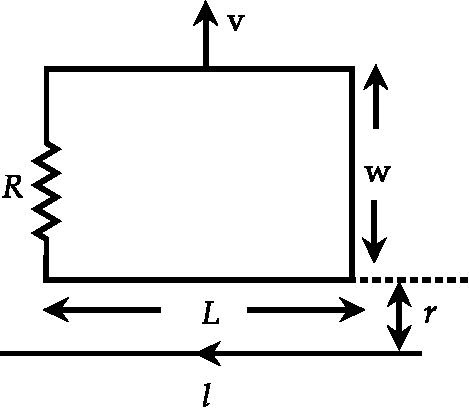
\includegraphics[height=3.5cm,width=4cm]{Ass-05}
	\end{figure}
	\item A square loop of side $L$ and mass $M$ is made of a wire of cross-sectional area $A$ and resistance $R$ The loop. moving with a constant velocity $v_{v} \hat{i}$ in the horizontal xy-plane, enters a region $0 \leq x \leq 2 L$ having constant magnetic field $B \hat{k}$
	\begin{figure}[H]
		\centering
		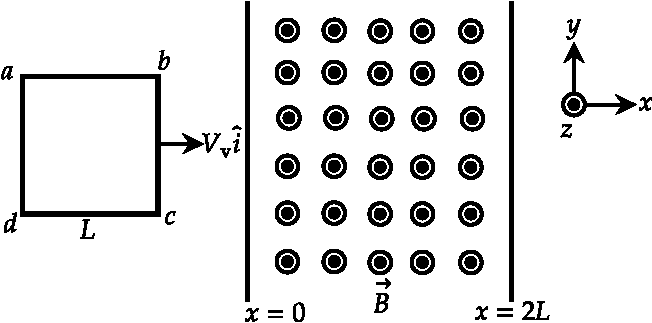
\includegraphics[height=4cm,width=8cm]{Ass-01}
	\end{figure}
	Find an expression for the $x$-component of the force $\vec{F}$ acting on the loop in terms of its velocity $\vec{v}(t), B, L$ and $R$.
	\item A coil of 15 turns, each of radius 1 centimeter, is rotating at a constant angular velocity $\omega=300$ radians per second in a uniform magnetic field of $0.5$ tesla, as shown in the figure. Assume at time $t=0$ that the normal $\hat{n}$ to the coil plane is along the $y$-direction and that the self-inductance of the coil can be neglected. If the coil resistance is 9 ohms, what will be the magnitude of the induced current in milliamperes?
	\begin{figure}[H]
		\centering
		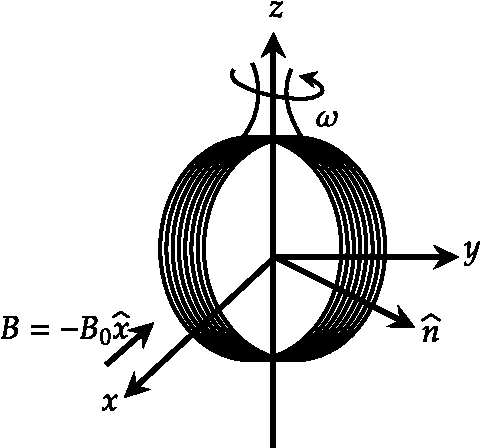
\includegraphics[height=3.8cm,width=4.3cm]{Ass-02}
	\end{figure}
	\item The circuit shown below is in a uniform magnetic lield that is into the page and is decreasing in magnitude at the rate of 150 Tesla/sec. Then tind the ammeter reading.
	\begin{figure}[H]
		\centering
		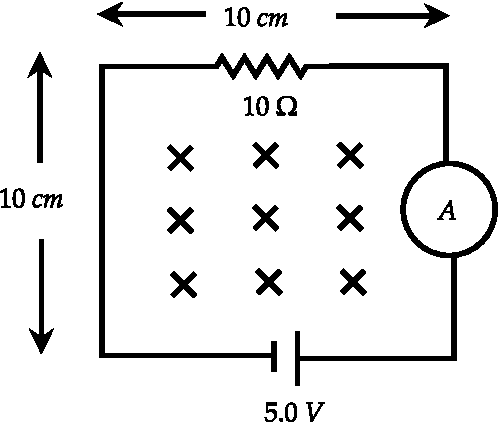
\includegraphics[height=4.5cm,width=5cm]{Ass-03}
	\end{figure}
	\item A parallel plate air-gap capacitor is made up of two plates of area $10 \mathrm{~cm}^{2}$ each kept at a distance of $0.88 \mathrm{~mm}$. A sine wave of amplitude $10 \mathrm{~V}$ and frequency $50 \mathrm{~Hz}$ is applied across the capacitor as shown in the figure.
	\begin{tasks}(1)
		\task[\textbf{a.}]Find the amplitude of the displacement current density between the plates.
		\task[\textbf{b.}]
		(b) Find the r.m.s value of the displacement current density between the plates.
		\task[\textbf{c.}]Find the average value of the displacement current density (in $\mathrm{mA} / \mathrm{m}^{2}$ ) between the plates.
	\end{tasks}
	\begin{figure}[H]
		\centering
		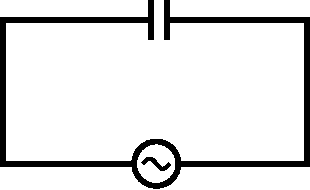
\includegraphics[height=2.5cm,width=4cm]{Ass-04}
	\end{figure}
	\item Consider a capacitor placed in free space, consisting of two concentric circular parallel plates of radii $r$. The separation $z$ between the plates oscillates with a constant frequency $\omega$, i.e. $z(t)=z_{0}+z_{1} \cos \omega t$. Here $z_{0}$ and $z_{1}\left(<z_{0}\right)$ are constants. The separation $z(t)$ $(<<r)$ is varied in such a way that the voltage $V_{0}$ across the capacitor remains constant,\\
	(a) Calculate the displacement current density and the displacement current between the plates through a concentric circle of radius $r / 2$.\\
	(b) Calculate the magnetic field vector $(\vec{H})$ between the plates at-a distance $r / 2$ from the axis of the capacitor.
\end{enumerate}

\newpage
\begin{abox}
Practise Set-2
\end{abox}
\begin{enumerate}
	\item  For constant uniform electric and magnetic field $\vec{E}=\vec{E}_{0}$ and $\vec{B}=\vec{B}_{0}$, it is possible to choose a gauge such that the scalar potential $\phi$ and vector potential $\vec{A}$ are given by
		{\exyear{NET/JRF(JUNE-2011)}}
		\begin{tasks}(1)
			\task[\textbf{A.}] $\phi=0$ and $\vec{A}=\frac{1}{2}\left(\vec{B}_{0} \times \vec{r}\right)$
			\task[\textbf{B.}] $\phi=-\vec{E}_{0} \cdot \vec{r}$ and $\vec{A}=\frac{1}{2}\left(\vec{B}_{0} \times \vec{r}\right)$
			\task[\textbf{C.}]  $\phi=-\vec{E}_{0} \cdot \vec{r}$ and $\vec{A}=0$
			\task[\textbf{D.}] $\phi=0$ and $\vec{A}=-\vec{E}_{0} t$
		\end{tasks}
	\item	Consider a solenoid of radius $R$ with $n$ turns per unit length, in which a time dependent current $I=I_{0} \sin \omega t$ (where $\left.\omega R / c<<1\right)$ flows. The magnitude of the electric field at a perpendicular distance $r<R$ from the axis of symmetry of the solenoid, is
		{\exyear{NET/JRF(DEC-2011)}}
		\begin{tasks}(2)
			\task[\textbf{A.}]  0
			\task[\textbf{B.}] $\frac{1}{2 r} \omega \mu_{0} n I_{0} R^{2} \cos \omega t$
			\task[\textbf{C.}] $\frac{1}{2} \omega \mu_{0} n I_{0} r \sin \omega t$
			\task[\textbf{D.}]  $\frac{1}{2} \omega \mu_{0} n I_{0} r \cos \omega t$
		\end{tasks}
\item	A constant electric current $I$ in an infinitely long straight wire is suddenly switched on at $t=0$. The vector potential at a perpendicular distance $r$ from the wire is given by $\vec{A}=\frac{\hat{k} \mu_{0} I}{2 \pi} \ln \left[\frac{1}{r}\left(c t+\sqrt{c^{2} t^{2}-r^{2}}\right)\right]$. The electric field at a distance $r(<c t)$ is
		{\exyear{NET/JRF(DEC-2011)}}
		\begin{tasks}(2)
			\task[\textbf{A.}] 0
			\task[\textbf{B.}] $\frac{\mu_{0} I}{2 \pi t} \frac{1}{\sqrt{2}}(\hat{i}-\hat{j})$
			\task[\textbf{C.}] $\frac{c \mu_{0} I}{2 \pi \sqrt{c^{2} t^{2}-r^{2}}} \frac{1}{\sqrt{2}}(\hat{i}+\hat{j})$
			\task[\textbf{D.}] $-\frac{c \mu_{0} I}{2 \pi \sqrt{c^{2} t^{2}-r^{2}}} \hat{k}$
		\end{tasks}
\item Consider an infinite conducting sheet in the $x y$-plane with a time dependent current density $K t \hat{i}$, where $K$ is a constant. The vector potential at $(x, y, z)$ is given by $\vec{A}=\frac{\mu_{0} K}{4 c}(c t-z)^{2} \hat{i}$. The magnetic field $\vec{B}$ is
	{	\exyear{NET/JRF(DEC-2012)}}
		\begin{tasks}(2)
			\task[\textbf{A.}] $\frac{\mu_{0} K t}{2} \hat{j}$
			\task[\textbf{B.}] $-\frac{\mu_{0} K z}{2 c} \hat{j}$
			\task[\textbf{C.}] $-\frac{\mu_{0} K}{2 c}(c t-z) \hat{i}$
			\task[\textbf{D.}] $-\frac{\mu_{0} K}{2 c}(c t-z) \hat{j}$
		\end{tasks}
\item A current $I$ is created by a narrow beam of protons moving in vacuum with constant velocity $\vec{u}$. The direction and magnitude, respectively of the Poynting vector $\vec{S}$ outside the beam at a radial distance $r$ (much larger than the width of the beam) from the axis, are
	{	\exyear{NET/JRF(JUNE-2013)}}
		\begin{tasks}(2)
			\task[\textbf{A.}] $\vec{S} \perp \vec{u}$ and $|\vec{S}|=\frac{I^{2}}{4 \pi^{2} \varepsilon_{0}|\vec{u}| r^{2}}$
			\task[\textbf{B.}] $\vec{S} \|(-\vec{u})$ and $|\vec{S}|=\frac{I^{2}}{4 \pi^{2} \varepsilon_{0}|\vec{u}| r^{4}}$
			\task[\textbf{C.}] $\vec{S} \| \vec{u}$ and $|\vec{S}|=\frac{I^{2}}{4 \pi^{2} \varepsilon_{0}|\vec{u}| r^{2}}$
			\task[\textbf{D.}] $\vec{S} \| \vec{u}$ and $|\vec{S}|=\frac{I^{2}}{4 \pi^{2} \varepsilon_{0}|\vec{u}| r^{4}}$
		\end{tasks}
	\item
		If the electric and magnetic fields are unchanged when the potential $\vec{A}$ changes (in suitable units) according to $\vec{A} \rightarrow \vec{A}+\hat{r}$, where $\vec{r}=r(t) \hat{r}$, then the scalar potential $\Phi$ must simultaneously change to
	{	\exyear{NET/JRF(JUNE-2013)}}
		\begin{tasks}(4)
			\task[\textbf{A.}] $\Phi-r$
			\task[\textbf{B.}] $\Phi+r$
			\task[\textbf{C.}] $\Phi-\partial \mathrm{r} / \partial t$
			\task[\textbf{D.}] $\Phi+\partial \mathrm{r} / \partial t$
		\end{tasks}
	\item
		Let $(V, \vec{A})$ and $\left(V^{\prime}, \overrightarrow{A^{\prime}}\right)$ denote two sets of scalar and vector potentials, and $\psi$ is a scalar function. Which of the following transformations leave the electric and magnetic fields (and hence Maxwell's equations) unchanged?
		{\exyear{NET/JRF(DEC-2013)}}
		\begin{tasks}(2)
			\task[\textbf{A.}] $\overrightarrow{A^{\prime}}=\vec{A}+\nabla \psi$ and $V^{\prime}=V-\frac{\partial \psi}{\partial t}$
			\task[\textbf{B.}] $\overrightarrow{A^{\prime}}=\vec{A}-\nabla \psi$ and $V^{\prime}=V+2 \frac{\partial \psi}{\partial t}$
			\task[\textbf{C.}] $\overrightarrow{A^{\prime}}=\vec{A}+\nabla \psi$ and $V^{\prime}=V+\frac{\partial \psi}{\partial t}$
			\task[\textbf{D.}] $\overrightarrow{A^{\prime}}=\vec{A}-\nabla \psi$ and $V^{\prime}=V-\frac{\partial \psi}{\partial t}$
		\end{tasks}
\item
		A time-dependent current $\vec{I}(t)=K t \hat{z}$ (where $K$ is a constant) is switched on at $t=0$ in an infinite current-carrying wire. The magnetic vector potential at a perpendicular distance $a$ from the wire is given (for time $t>a / c$ ) by
	{	\exyear{NET/JRF(JUNE-2014)}}
		\begin{tasks}(2)
			\task[\textbf{A.}]  $\hat{z} \frac{\mu_{0} K}{4 \pi c} \int_{-\sqrt{c^{2} t^{2}-a^{2}}}^{\sqrt{c^{2} t^{2}-a^{2}}} d z \frac{c t-\sqrt{a^{2}+z^{2}}}{\left(a^{2}+z^{2}\right)^{1 / 2}}$
			\task[\textbf{B.}]  $\hat{z} \frac{\mu_{0} K}{4 \pi} \int_{-c t}^{c t} d z \frac{t}{\left(a^{2}+z^{2}\right)^{1 / 2}}$
			\task[\textbf{C.}] $\hat{z} \frac{\mu_{0} K}{4 \pi c} \int_{-c t}^{c t} d z \frac{c t-\sqrt{a^{2}+z^{2}}}{\left(a^{2}+z^{2}\right)^{1 / 2}}$
			\task[\textbf{D.}] $\hat{z} \frac{\mu_{0} K}{4 \pi} \int_{-\sqrt{c^{2} t^{2}-a^{2}}}^{\sqrt{c^{2} t^{2}-a^{2}}} d z \frac{t}{\left(a^{2}+z^{2}\right)^{1 / 2}}$
		\end{tasks}
	
	
	
	
	
	\item A current $i_{p}$ flows through the primary coil of a transformer. The graph of $i_{p}(t)$ as a function of time $t$ is shown in the figure below.\\
	\begin{figure}[H]
		\centering
		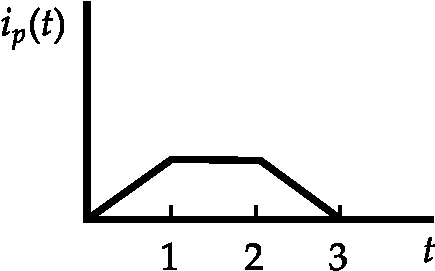
\includegraphics[height=3cm,width=5cm]{diagram-20211011(27)-crop}
	\end{figure}
	Which of the following graphs represents the current $i_{S}$ in the secondary coil?
	{\exyear{NET/JRF(JUNE-2014)}}
	\begin{tasks}(2)
		\task[\textbf{A.}] \begin{figure}[H]
			\centering
			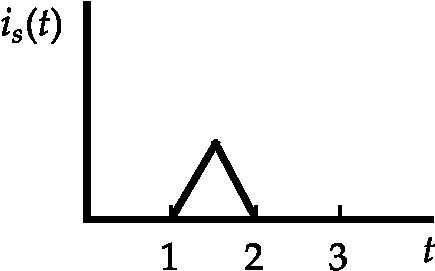
\includegraphics[height=3cm,width=5cm]{diagram-20211011(28)-crop}
		\end{figure}
		\task[\textbf{B.}] \begin{figure}[H]
			\centering
			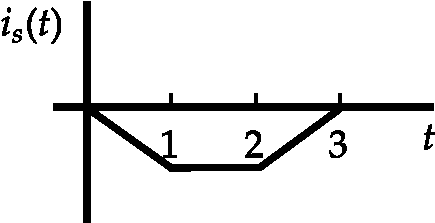
\includegraphics[height=3cm,width=5cm]{diagram-20211011(29)-crop}
		\end{figure}
		\task[\textbf{C.}] \begin{figure}[H]
			\centering
			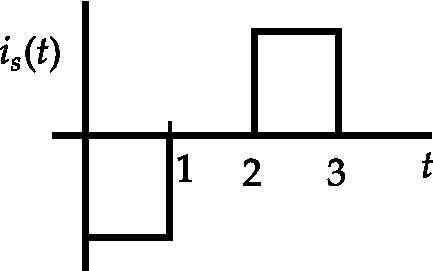
\includegraphics[height=3cm,width=5cm]{diagram-20211011(30)-crop}
		\end{figure}
		\task[\textbf{D.}] \begin{figure}[H]
			\centering
			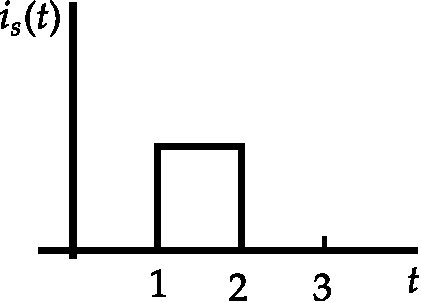
\includegraphics[height=3cm,width=5cm]{diagram-20211011(31)-crop}
		\end{figure}
	\end{tasks}
	\begin{answer}
		\begin{align*}
		i_{s} \propto-\frac{d i_{p}}{d t}
		\end{align*}
		So the correct answer is \textbf{Option (C)}
	\end{answer}
	\item Suppose the $y z$-plane forms a chargeless boundary between two media of permittivities $\epsilon_{\text {left }}$ and $\epsilon_{\text {right }}$ where $\epsilon_{\text {left }}: \epsilon_{\text {right }}=1: 2$, if the uniform electric field on the left is $\vec{E}_{\text {left }}=c(\hat{i}+\hat{j}+\hat{k})$ (where $c$ is a constant), then the electric field on the right $\vec{E}_{\text {right }}$ is
	{\exyear{NET/JRF(JUNE-2015)}}
	\begin{tasks}(4)
		\task[\textbf{A.}]  $c(2 \hat{i}+\hat{j}+\hat{k})$
		\task[\textbf{B.}] $c(\hat{i}+2 \hat{j}+2 \hat{k})$
		\task[\textbf{C.}] $c\left(\frac{1}{2} \hat{i}+\hat{j}+\hat{k}\right)$
		\task[\textbf{D.}] $c\left(\hat{i}+\frac{1}{2} \hat{j}+\frac{1}{2} \hat{k}\right)$
	\end{tasks}
	\begin{answer}$\left. \right. $
		\begin{figure}[H]
			\centering
			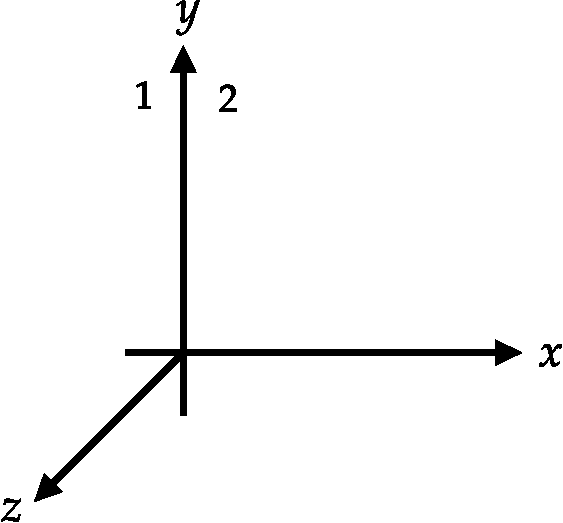
\includegraphics[height=4cm,width=4.5cm]{diagram-20211011(34)-crop}
		\end{figure}
		\begin{align*}
		E_{1}^{\prime \prime}&=c(\hat{j}+\hat{k})=E_{2}^{\prime \prime}\\
		D_{1}^{\perp}&=D_{2}^{\perp} \Rightarrow \epsilon_{1} E_{1}^{\perp}=\epsilon_{2} E_{2}^{\perp} \Rightarrow E_{2}^{1}=\frac{\epsilon_{1}}{\epsilon_{2}} E_{1}^{\perp}\\
		\Rightarrow E_{2}^{\perp}&=\frac{1}{2} c \hat{i} \Rightarrow \vec{E}_{2}=c\left(\frac{1}{2} \hat{i}+\hat{j}+\hat{k}\right)
		\end{align*}
		So the correct answer is \textbf{Option (C)}
	\end{answer}
	\item  The half space region $x>0$ and $x<0$ are filled with dielectric media of dielectric constants $\varepsilon_{1}$ and $\varepsilon_{2}$ respectively. There is a uniform electric field in each part. In the right half, the electric field makes an angle $\theta_{1}$ to the interface. The corresponding angle $\theta_{2}$ in the left half satisfies
	{{\exyear{NET/JRF(JUNE-2016)}}}
	\begin{figure}[H]
		\centering
		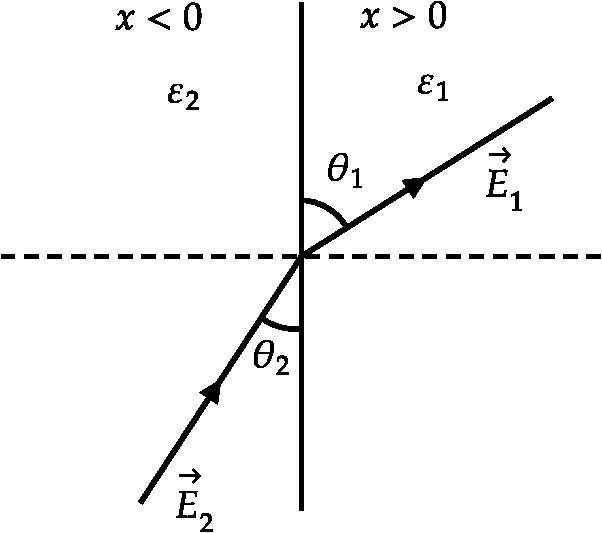
\includegraphics[height=4cm,width=5cm]{diagram-20211011(41)-crop}
	\end{figure}
	\begin{tasks}(2)
		\task[\textbf{A.}] $\varepsilon_{1} \sin \theta_{2}=\varepsilon_{2} \sin \theta_{1}$
		\task[\textbf{B.}] $\varepsilon_{1} \tan \theta_{2}=\varepsilon_{2} \tan \theta_{1}$
		\task[\textbf{C.}] $\varepsilon_{1} \tan \theta_{1}=\varepsilon_{2} \tan \theta_{2}$
		\task[\textbf{D.}] $\varepsilon_{1} \sin \theta_{1}=\varepsilon_{2} \sin \theta_{2}$
	\end{tasks}
	\begin{answer}
		\begin{align*}
		\frac{\tan \theta_{1}}{\tan \theta_{2}}&=\frac{\frac{E_{1}^{\perp}}{E_{1}^{\|}}}{\frac{E_{2}^{\perp}}{E_{2}^{\|}}}=\frac{E_{1}^{\perp}}{E_{2}^{\perp}} \quad\left(\because E_{1}^{\|}=E_{2}^{\|}\right)\\
		D_{1}^{\perp}&=D_{2}^{\perp} \Rightarrow \varepsilon_{1} E_{1}^{\perp}=\varepsilon_{2} E_{2}^{\perp} \Rightarrow \frac{E_{1}^{\perp}}{E_{2}^{\perp}}=\frac{\varepsilon_{2}}{\varepsilon_{1}} \Rightarrow \frac{\tan \theta_{1}}{\tan \theta_{2}}\\&=\frac{\varepsilon_{2}}{\varepsilon_{1}} \Rightarrow \varepsilon_{1} \tan \theta_{1}=\varepsilon_{2} \tan \theta_{2}
		\end{align*}
		So the correct answer is \textbf{Option (C)}
	\end{answer}
	\item A magnetic field $B$ is $B \hat{z}$ in the region $x>0$ and zero elsewhere. A rectangular loop, in the $x y$-plane, of sides $l$ (along the $x$-direction) and $h$ (along the $y$ - direction) is inserted into the $x>0$ region from the $x<0$ region at constant velocity $v=v \hat{x}$. Which of the following values of $l$ and $h$ will generate the largest EMF?
	{\exyear{NET/JRF(JUNE-2016)}}
	\begin{tasks}(2)
		\task[\textbf{A.}] $l=8, h=3$
		\task[\textbf{B.}] $l=4, h=6$
		\task[\textbf{C.}] $l=6, h=4$
		\task[\textbf{D.}] $l=12, h=2$
	\end{tasks}
	\begin{answer}$\left. \right. $
		\begin{figure}[H]
			\centering
			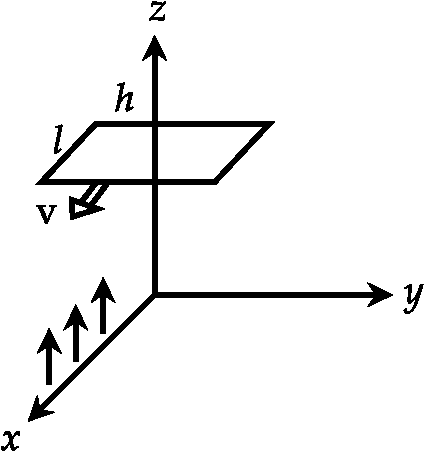
\includegraphics[height=4cm,width=5cm]{diagram-20211011(42)-crop}
		\end{figure}
		\begin{align*}
		\phi_{m} \propto B h x\\
		\varepsilon \propto \frac{-d \phi_{m}}{d t} \propto B v h \propto h
		\end{align*}
		So the correct answer is \textbf{Option (B)}
	\end{answer}
	\item The vector potential $\vec{A}=k e^{-a t} r \hat{r}$ (where $a$ and $k$ are constants) corresponding to an electromagnetic field is changed to $\overrightarrow{A^{\prime}}=-k e^{-a t} r \hat{r}$. This will be a gauge transformation if the corresponding change $\phi^{\prime}-\phi$ in the scalar potential is
	{\exyear{NET/JRF(JUNE-2017)}}
	\begin{tasks}(4)
		\task[\textbf{A.}] $a k r^{2} e^{-a t}$
		\task[\textbf{B.}] $2 a k r^{2} e^{-a t}$
		\task[\textbf{C.}] $-a k r^{2} e^{-a t}$
		\task[\textbf{D.}] $-2 a k r^{2} e^{-a t}$
	\end{tasks}
	\begin{answer}
		\begin{align*}
		\intertext{Gauge TransformationGauge Transformation}
		\vec{A}&=\vec{A}+\vec{\nabla} \lambda, \phi^{\prime}=\phi-\frac{\partial \lambda}{\partial t} \Rightarrow \vec{A}-\vec{A}\\&=-2 k e^{-a t} r \hat{r}=\vec{\nabla} \lambda=\frac{\partial \lambda}{\partial r} \hat{r}\\
		\Rightarrow \lambda&=-k e^{-a t} r^{2} \Rightarrow \frac{\partial \lambda}{\partial t}=k a e^{-a t} r^{2}\\
		\Rightarrow \phi^{\prime}-\phi&=-\frac{\partial \lambda}{\partial t}=-k a e^{-a t} r^{2}
		\end{align*}
		So the correct answer is \textbf{Option (C)}
	\end{answer}
	\item The charge distribution inside a material of conductivity $\sigma$ and permittivity $\in$ at ini time $t=0$ is $\rho(r, 0)=\rho_{0}$, a constant. At subsequent times $\rho(r, t)$ is given by
	{\exyear{NET/JRF(JUNE-2017)}}
	\begin{tasks}(2)
		\task[\textbf{A.}]  $\rho_{0} \exp \left(-\frac{\sigma t}{\epsilon}\right)$
		\task[\textbf{B.}] $\frac{1}{2} \rho_{0}\left[1+\exp \left(\frac{\sigma t}{\in}\right)\right]$
		\task[\textbf{C.}]  $\frac{\rho_{0}}{\left[1-\exp \left(\frac{\sigma t}{\epsilon}\right)\right]}$
		\task[\textbf{D.}] $\rho_{0} \cosh \frac{\sigma t}{\in}$
	\end{tasks}
	\begin{answer}
		\begin{align*}
		\vec{J}_{f}&=\sigma \vec{E}, \vec{\nabla} \cdot \vec{E}=\frac{\rho_{f}}{\in}, \quad \vec{\nabla} \cdot \vec{J}_{f}=-\frac{\partial \rho_{f}}{\partial E}\\
		\Rightarrow \sigma \vec{\nabla} \cdot \vec{E}&=-\frac{\partial \rho_{f}}{\partial t} \Rightarrow \frac{\partial \rho_{f}}{\partial t}=-\frac{\sigma}{\epsilon} \rho_{f}\\
		\Rightarrow \rho_{f}(t)&=\rho_{0} \exp \left(\frac{-\sigma}{\epsilon} \rho_{f}\right) \Rightarrow \rho_{f}(t)=\rho_{0} \exp \left(\frac{-\sigma}{\epsilon} t\right)
		\end{align*}
		So the correct answer is \textbf{Option (A)}
	\end{answer}
	\item  The electric field $\vec{E}$ and the magnetic field $\vec{B}$ corresponding to the scalar and vector potentials, $V(x, y, z, t)=0$ and $\vec{A}(x, y, z, t)=\frac{1}{2} \hat{k} \mu_{0} A_{0}(c t-x)$, where $A_{0}$ is a constant, are 
	{\exyear{NET/JRF(JUNE-2018)}}
	\begin{tasks}(2)
		\task[\textbf{A.}] (a) $\vec{E}=0$ and $\vec{B}=\frac{1}{2} \hat{j} \mu_{0} A_{0}$
		\task[\textbf{B.}] $\vec{E}=-\frac{1}{2} \hat{k} \mu_{0} A_{0} c$ and $\vec{B}=\frac{1}{2} \hat{j} \mu_{0} A_{0}$
		\task[\textbf{C.}]  $\vec{E}=0$ and $\vec{B}=-\frac{1}{2} \hat{i} \mu_{0} A_{0}$
		\task[\textbf{D.}] $\vec{E}=\frac{1}{2} \hat{k} \mu_{0} A_{0} c$ and $\vec{B}=-\frac{1}{2} \hat{i} \mu_{0} A_{0}$
	\end{tasks}
	\begin{answer}
		\begin{align*}
		\vec{E}&=\frac{-\partial \vec{A}}{\partial t}=-\left[\frac{1}{2} \mu_{0} A_{0}(c-0)\right] \hat{k}=-\frac{1}{2} \mu_{0} A_{0} c \hat{k}\\
		\vec{B}&=\vec{\nabla} \times \vec{A}=\left|\begin{array}{ccc}\hat{x} & \hat{y} & \hat{z} \\ \frac{\partial}{\partial x} & \frac{\partial}{\partial y} & \frac{\partial}{\partial z} \\ 0 & 0 & A_{z}\end{array}\right|\\&=\hat{x} \frac{\partial A_{z}}{\partial y}-\hat{y} \frac{\partial A_{z}}{\partial x} \Rightarrow \vec{B}=\frac{1}{2} \mu_{0} A_{0} \hat{j}
		\end{align*}
		So the correct answer is \textbf{Option (B)}
	\end{answer}
	\item Which of the following is not a correct boundary condition at an interface between two homogeneous dielectric media? (In the following $\hat{n}$is a unit vector normal to the  interface, $\sigma$ and $\vec{j}_s$, are the surface charge and current densities, respectively.)
	{\exyear{NET/JRF(JUNE-2019)}}
	\begin{tasks}(2)
		\task[\textbf{A.}] $\hat{n} \times\left(\vec{D}_{1}-\vec{D}_{2}\right)=0$
		\task[\textbf{B.}] $\hat{n} \times\left(\vec{H}_{1}-\vec{H}_{2}\right)=\vec{j}_{s}$
		\task[\textbf{C.}] $\hat{n} \cdot\left(\vec{D}_{1}-\vec{D}_{2}\right)=\sigma$
		\task[\textbf{D.}] $\hat{n} \cdot\left(\vec{B}_{1}-\vec{B}_{2}\right)=0$
	\end{tasks}
	\begin{answer}
		\begin{align*}
		\intertext{Since media is homogeneous dielectric:
			assume uniform polarisation and
			magnetisation.}
		\intertext{$\sigma$ and $\vec{j }_s$ , are the free surface charge and free surface current densities.}
		\vec{\nabla} \times \vec{D}&=0 \quad \Rightarrow D_{1}^{\|}=D_{2}^{\|} \\ \because \vec{\nabla} \times \vec{P}&=0 \quad\text{ and }\quad D_{1}^{\perp}-D_{2}^{\perp}=\sigma\\
		\text{Thus }\left(\vec{D}_{1}-\vec{D}_{2}\right)&=\sigma \hat{n}\\
		\Rightarrow \hat{n} \cdot\left(\vec{D}_{1}-\vec{D}_{2}\right)&=\sigma \quad\text{ and } \hat{n} \times\left(\vec{D}_{1}-\vec{D}_{2}\right) \neq 0\\
		\vec{\nabla} \cdot \vec{H}&=-\vec{\nabla} \cdot \vec{M}=0 \quad \Rightarrow H_{1}^{\perp}=H_{2}^{\perp} \\ \because \vec{\nabla} \cdot \vec{M}&=0 \quad\text{ and } \quad H_{1}^{\|}-H_{2}^{\|}=j_{s}\\
		\text{	Thus }\left(\vec{H}_{1}-\vec{H}_{2}\right)=\vec{j}_{s} \times \hat{n}\\
		\Rightarrow \hat{n} \times\left(\vec{H}_{1}-\vec{H}_{2}\right)&=\vec{j}_{s}\\
		\text{Also}
		\intertext{$\vec{\nabla} \cdot \vec{B}=0 \quad \Rightarrow B_{1}^{\perp}=B_{2}^{\perp} \quad$ and $\quad B_{1}^{\|}-B_{1}^{\|}=\mu_{0} K$ (assume $K$ is total surface current at interface)}\\
		\text{Thus }\left(\vec{B}_{1}-\vec{B}_{2}\right)&=\mu_{0}(\vec{K} \times \hat{n}) .\\
		\Rightarrow \hat{n} \cdot\left(\vec{B}_{1}-\vec{B}_{2}\right)&=0
		\end{align*}
		So the correct answer is \textbf{Option (A)}
	\end{answer}
\end{enumerate}
\newpage
\begin{abox}
	Previous year solutions
	\end{abox}
\begin{enumerate}
	\begin{minipage}{\textwidth}
		\item  The electric and the magnetic field $\vec{E}(z, t)$ and $\vec{B}(z, t)$, respectively corresponding to the scalar potential $\phi(z, t)=0$ and vector potential $\vec{A}(z, t)=\hat{i} t z$ are
		\exyear{GATE 2012}
	\end{minipage}
	\begin{tasks}(2)
		\task[\textbf{A.}] $\vec{E}=\hat{i} z$ and $\vec{B}=-\hat{j} t$
		\task[\textbf{B.}]$\vec{E}=\hat{i} z$ and $\vec{B}=\hat{j t}$
		\task[\textbf{C.}]$\vec{E}=-\hat{i} z$ and $\vec{B}=-\hat{j t}$
		\task[\textbf{D.}]$\vec{E}=-\hat{i} z$ and $\vec{B}=-\hat{j} \mathrm{t}$
	\end{tasks}
\begin{answer}
	$\vec{E}=-\vec{\nabla} \phi-\frac{\partial \vec{A}}{\partial t}=-\frac{\partial \vec{A}}{\partial t}=-\hat{i} z, \vec{B}=\vec{\nabla} \times \vec{A}=+\hat{j} t$\\
The correct option is \textbf{(d)}
\end{answer}
\begin{minipage}{\textwidth}
	\item If the vector potential $\vec{A}=\alpha x \hat{x}+2 y \hat{y}-3 z \hat{z}$, satisfies the Coulomb gauge, the value of the constant $\alpha$ is
	\exyear{GATE 2015}
\end{minipage}
\begin{answer}
$$\text { Coulomb gauge condition } \vec{\nabla} \cdot \vec{A}=0 \Rightarrow \alpha+2-3=0 \Rightarrow \alpha=1$$	
\end{answer}
\begin{minipage}{\textwidth}
	\item Consider magnetic vector potential $\tilde{A}$ and scalar potential $\Phi$ which define the magnetic field $\vec{B}$ and electric field $\vec{E}$. If one adds $\vec{\nabla} \lambda$ to $\vec{A}$ for a well-defined $\lambda$, then what should be added to $\Phi$ so that $\vec{E}$ remains unchanged up to an arbitrary function of time, $f(t)$ ?
	\exyear{JEST 2017}
\end{minipage}
\begin{tasks}(2)
	\task[\textbf{A.}] $\frac{\partial \lambda}{\partial t}$
	\task[\textbf{B.}]$-\frac{\partial \lambda}{\partial t}$
	\task[\textbf{C.}]$\frac{1}{2} \frac{\partial \lambda}{\partial t}$
	\task[\textbf{D.}]$-\frac{1}{2} \frac{\partial \lambda}{\partial t}$
\end{tasks}
\begin{answer}
Consider Gauge Transformation
$$
\vec{A}^{\prime}=\vec{A}-\vec{\nabla} \lambda=\vec{A}+\vec{V}(-\lambda) \quad \text { and } \quad \Phi^{\prime}=\Phi-\frac{\partial(-\lambda)}{\partial t}=\Phi+\frac{\partial \lambda}{\partial t}
$$
The correct option is \textbf{(a)}	
\end{answer}
\end{enumerate}






























